%%%%%%%% ICML 2026 WORKSHOP SUBMISSION %%%%%%%%%%%%%%%%%

\documentclass{article}

\usepackage{microtype}
\usepackage{graphicx}
\usepackage{subcaption}
\usepackage{booktabs}
\usepackage{hyperref}
\newcommand{\theHalgorithm}{\arabic{algorithm}}
\usepackage{../icml2026/icml2026}
\usepackage{amsmath}
\usepackage{amssymb}
\usepackage{mathtools}
\usepackage[capitalize,noabbrev]{cleveref}

\icmltitlerunning{\raisebox{-1.5pt}{\fontsize{7}{7}\selectfont PatchSteg}}

\begin{document}

\twocolumn[
  \icmltitle{PatchSteg: Probing Spatially Localized Information Preservation in Diffusion VAE Latents}

  \begin{icmlauthorlist}
    \icmlauthor{Anonymous Authors}{anon}
  \end{icmlauthorlist}

  \icmlaffiliation{anon}{Anonymous Institution}
  \icmlcorrespondingauthor{Anonymous Author}{anonymous@example.com}
  \icmlkeywords{mechanistic interpretability, autoencoders, latent representations, steganography, generative models}

  \vskip 0.3in
]

\printAffiliationsAndNotice{}

\begin{abstract}
We study whether information inserted into the latent representation of a pretrained diffusion VAE survives a decode--reencode round trip, and use this as an intervention-based probe of latent stability. We introduce PatchSteg, a simple training-free probe that encodes bits by adding signed perturbations to selected spatial latent positions and decodes them from the re-encoded image. Across Stable Diffusion VAE backbones, recovery is highly non-uniform across spatial positions and strongly content-dependent: textured images support reliable recovery while smooth images do not. Reconstruction error does not explain carrier quality; instead, local image statistics and encode--decode geometry better predict which positions preserve perturbation direction. These findings reveal a concrete representation-level failure mode for monitoring image-mediated model communication while providing a quantitative probe for studying information preservation in generative autoencoders.
\end{abstract}

\section{Introduction}

Mechanistic interpretability often studies neural networks by intervening on internal states and observing whether the induced information is used, erased, or transformed. For generative image models, pretrained autoencoders are a natural target for this style of analysis: diffusion pipelines rely on VAE latents as compressed internal states, yet comparatively little is known about which local latent perturbations survive when mapped through image space and encoded again.

We ask a concrete question: when a latent vector $z$ is locally perturbed, decoded to an image, and re-encoded, which parts of the perturbation remain recoverable? We operationalize this through a deliberately simple bit-recovery probe, PatchSteg. At a selected spatial latent position, a bit is written by adding either $+\epsilon d$ or $-\epsilon d$ along a shared direction $d\in\mathbb{R}^4$. A receiver re-encodes the resulting image and reads the bit from the sign of the projected displacement. Successful decoding means that the composite map $\mathrm{Enc}\circ\mathrm{Dec}$ preserves the sign of a local directional intervention.

The security motivation is model-to-model communication through shared images. If internal-state perturbations can survive through visually innocuous images, then image-mediated monitoring may miss information that is legible to another model using the same representation. For this workshop paper, however, we treat covert communication primarily as a measurement tool: it converts latent preservation into a bit accuracy, stability, and rate--distortion signal that can be compared across positions, images, directions, and VAE backbones.

Our contributions are:
\begin{enumerate}
    \item We introduce PatchSteg, a training-free intervention probe for measuring local information preservation in diffusion VAE latents through decode--reencode bit recovery.
    \item We show that latent stability is spatially non-uniform, content-dependent, and not explained by reconstruction error alone, with evidence across synthetic images, 300 CIFAR-10 images, and multiple VAE backbones.
    \item We characterize the safety implication: stable latent directions instantiate a bounded covert channel, while detection and sanitization experiments expose a reliability--stealth--fidelity tradeoff.
\end{enumerate}

\begin{figure*}[t]
\centering
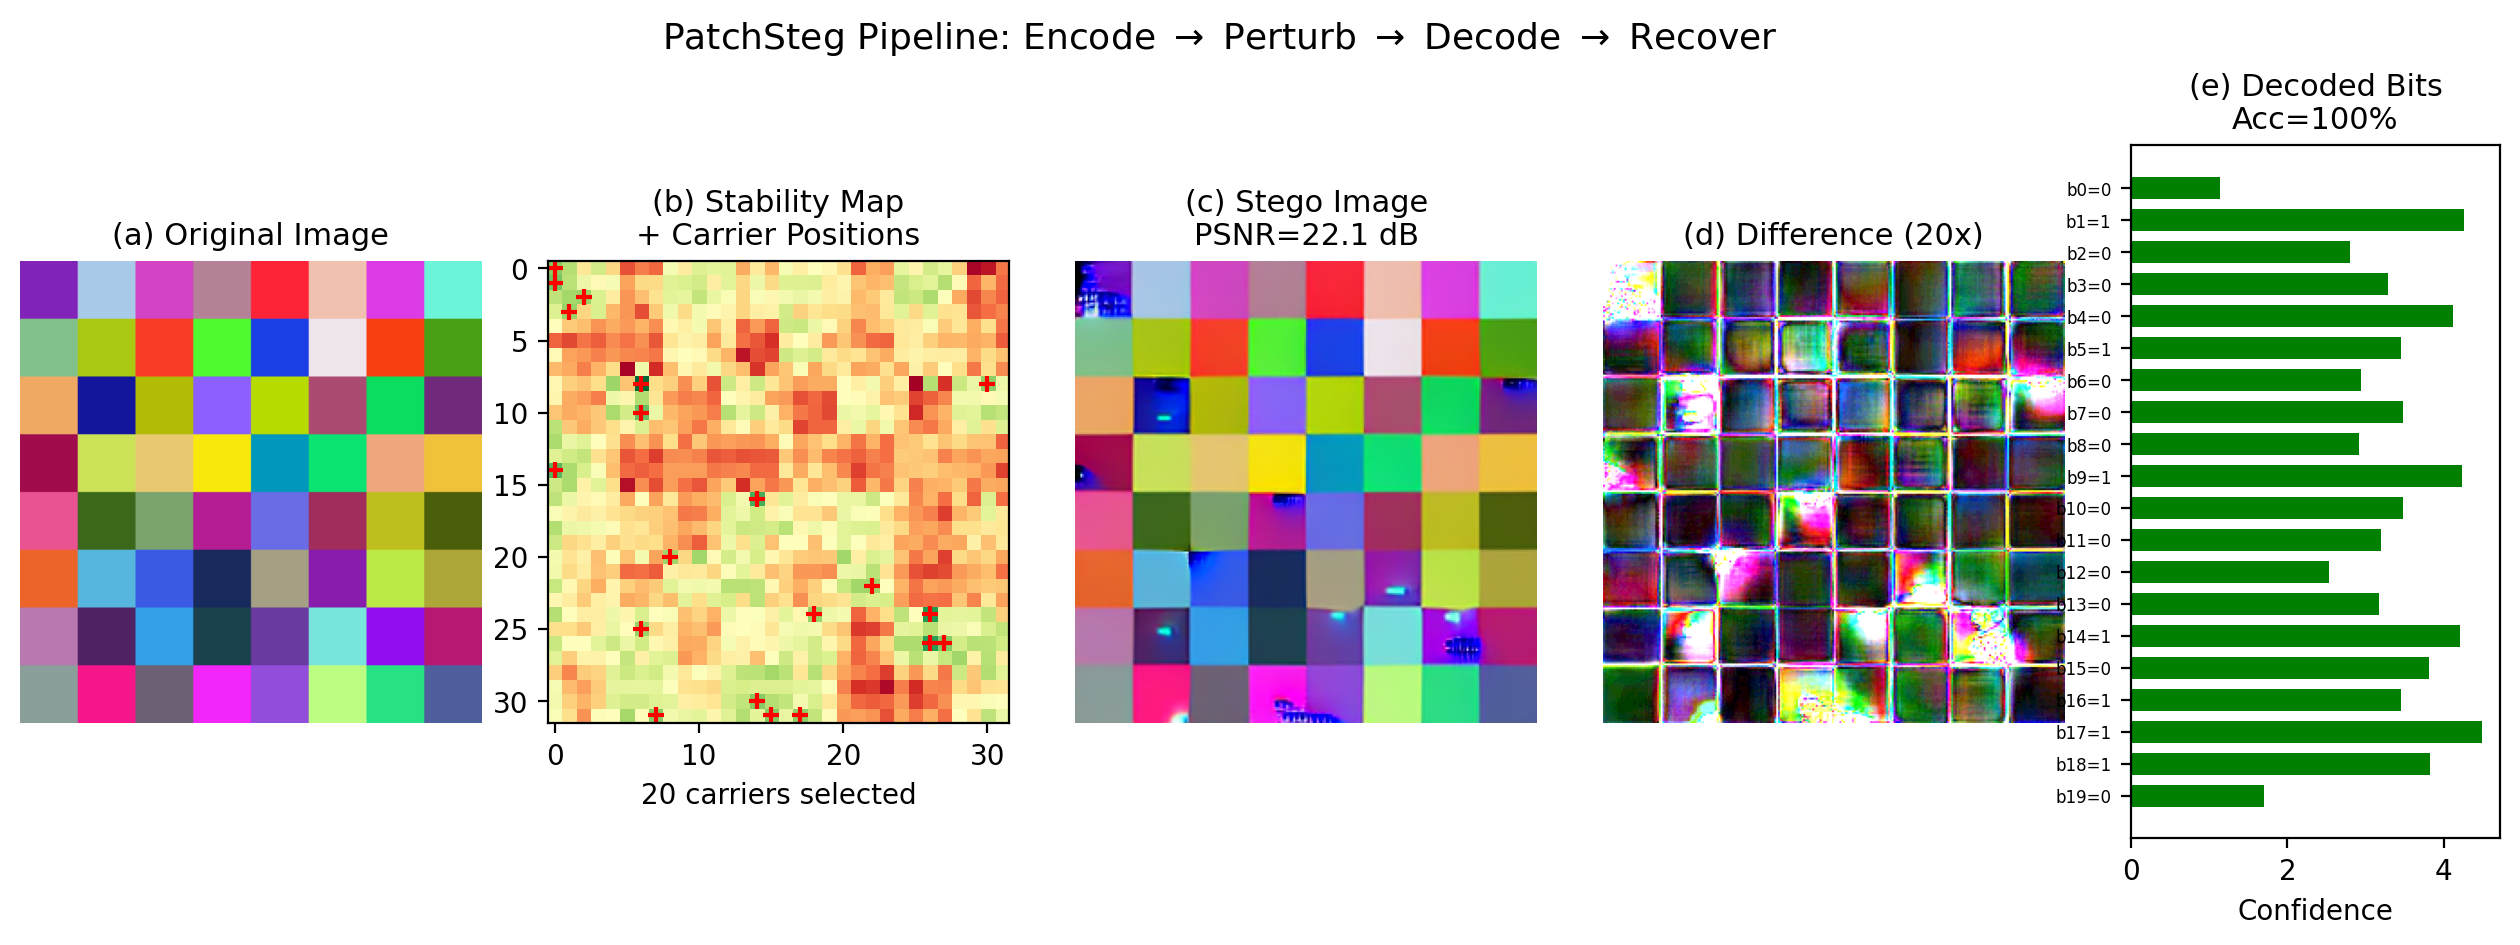
\includegraphics[width=0.93\textwidth]{figures/hero_pipeline.png}
\caption{PatchSteg as a latent-stability probe. A local signed perturbation is written into the VAE latent, decoded to image space, and read after re-encoding. Recovery of the bit indicates that the local perturbation direction survived the round trip through pixels.}
\label{fig:hero}
\end{figure*}

\section{Related Work}

\textbf{Mechanistic analysis of generative representations.}
Our work is closest in spirit to intervention-based interpretability: instead of only measuring reconstruction quality, we ask whether local information inserted into a representation is preserved by the model's computation. Prior work shows that VAE latent spaces exhibit structured geometry, including principal-component-like directions \citep{rolinek2019variational}. PatchSteg uses bit recovery as a direct behavioral probe of such geometry in pretrained diffusion VAEs.

\textbf{Neural image steganography and watermarking.}
RoSteALS trains encoder--decoder components for robust latent steganography \citep{bui2023rosteals}. Stable Signature \citep{fernandez2023stable}, Tree-Ring Watermarking \citep{wen2023treering}, and Gaussian Shading \citep{yang2024gaussian} watermark generated images, often by controlling generation-time noise or model parameters. PSyDUCK studies training-free steganography for latent diffusion models using generation-time trajectory control \citep{jiang2025psyduck}. PatchSteg differs in its post-hoc setting: it edits the latent of an existing image and uses no training. We use these connections to motivate the probe and defer broad steganographic claims to carefully bounded experiments.

\textbf{Covert channels and AI monitoring.}
Recent work on secret collusion among language-model agents demonstrates that model outputs can carry hidden messages that are difficult for human monitors to recognize \citep{motwani2024secret}. Images are a plausible communication substrate for multimodal agents. PatchSteg makes this substrate concrete for VAE-based vision systems, but the interpretability question is broader: which internal perturbations remain legible after passing through an apparently benign external medium?

\section{PatchSteg Probe}
\label{sec:method}

\subsection{Backbone And Latents}

Our primary backbone is the Stable Diffusion VAE checkpoint \texttt{stabilityai/sd-vae-ft-mse}. For an $H\times H$ input image, the encoder produces a latent tensor $z\in\mathbb{R}^{4\times H/8\times H/8}$. We follow the checkpoint convention and apply the VAE scaling factor during encode and decode. Unless otherwise stated, images are resized to $256\times256$, yielding a $4\times32\times32$ latent grid. We also test SD-VAE-EMA and SDXL-VAE to check whether the phenomenon is checkpoint-specific.

\subsection{Writing And Reading Bits}

Given a seed $s$, sender and receiver derive a unit direction $d\in\mathbb{R}^4$ and a carrier set $\mathcal{C}=\{(r_i,c_i)\}_{i=1}^K$. For bit $b_i\in\{0,1\}$, PatchSteg writes:
\begin{equation}
    z_{:,r_i,c_i}^{\,\mathrm{stego}}
    =
    z_{:,r_i,c_i}
    +
    (2b_i-1)\epsilon d ,
\end{equation}
where $\epsilon$ controls intervention strength. The modified latent is decoded to the stego image.

The receiver re-encodes the stego image to $z'$ and compares it to a clean round-trip baseline $\bar z=\mathrm{Enc}(\mathrm{Dec}(z))$:
\begin{equation}
    \hat b_i =
    \mathbb{1}\left[
    \langle z'_{:,r_i,c_i}-\bar z_{:,r_i,c_i}, d\rangle > 0
    \right].
\end{equation}
The clean baseline removes systematic reconstruction drift. This means the baseline protocol studies a shared-cover setting: both agents can derive the same cover latent or clean round-trip baseline. A blind variant based on distribution matching is discussed as exploratory material in \cref{sec:extensions}.

\subsection{Stability Score}

For an image $x$, position $(r,c)$, direction $d$, and strength $\epsilon$, define the directional stability:
\begin{equation}
\label{eq:stability}
S_{r,c}(x;d,\epsilon)
=
\left\langle
\mathrm{Enc}(\mathrm{Dec}(z+\epsilon d_{r,c}))_{:,r,c}
-
\bar z_{:,r,c},
d
\right\rangle ,
\end{equation}
where $d_{r,c}$ denotes a perturbation applied only at spatial position $(r,c)$. Positive $S$ means the sign of the intervention survives the round trip. Larger $|S|$ gives a higher-margin carrier.

In practice we estimate a stability map by perturbing positions, measuring projected survival after decode--reencode, and ranking positions by margin. Stability-selected carriers allow the same bit-recovery probe to test whether high-scoring positions causally support more reliable communication than random positions.

\section{Experimental Setup}

\textbf{Datasets.}
We use synthetic images to isolate structure (solid colors, gradients, color blocks, checkerboards, noise, and sine patterns) and natural images from CIFAR-10. The largest natural-image evaluation uses 300 CIFAR-10 images, 30 per class, resized to $256\times256$. We report this explicitly because upscaling low-resolution images is a limitation for claims about native high-resolution photography.

\textbf{Metrics.}
The primary interpretability metric is bit accuracy: the fraction of local intervention signs recovered after decode--reencode. We also report PSNR as a distortion measure, and use stability maps, per-image capacity, detector AUC, and robustness under image transformations as secondary measurements.

\textbf{Detectors.}
To bound the monitoring risk, we evaluate simple latent-statistics logistic regression, latent residual features, pixel residual features, spectral features, and small MLPs. Detector results are detector- and protocol-specific; we do not claim broad undetectability.

\section{Results}

\subsection{Local Latent Interventions Survive Round Trips}

Directional perturbations can survive the full encode--perturb--decode--reencode pipeline. With random carriers, recovery improves sharply as $\epsilon$ increases; with 20 carriers at $256\times256$, the baseline probe reaches 100\% bit accuracy at $\epsilon=5.0$ while maintaining PSNR above 30 dB. At $\epsilon=2.0$, random-carrier accuracy is lower, motivating explicit carrier-stability measurement.

\begin{table}[t]
\caption{Round-trip validation with random carrier selection at $256\times256$. Bit recovery measures whether the sign of the local latent intervention survives through image space.}
\label{tab:roundtrip}
\centering
\begin{small}
\begin{tabular}{cccc}
\toprule
$\epsilon$ & Carriers & Bit Acc. (\%) & PSNR (dB) \\
\midrule
0.5 & 5  & 80.0  & 32.0 \\
0.5 & 20 & 52.5  & 32.0 \\
2.0 & 5  & 90.0  & 31.8 \\
2.0 & 20 & 75.0  & 31.7 \\
5.0 & 5  & 100.0 & 31.4 \\
5.0 & 20 & 100.0 & 30.7 \\
\bottomrule
\end{tabular}
\end{small}
\end{table}

\subsection{Carrier Stability Is Spatially Non-Uniform}

\Cref{fig:stability} shows that stability varies across the latent grid. Averaged stability scores at $\epsilon=5.0$ range from 0.98 to 3.48 across positions, and selecting high-margin carriers substantially improves recovery at lower perturbation strengths. On a structured color-block image, stability-selected carriers at $\epsilon=2.0$ achieve 100\% bit accuracy with 20 carriers, compared with 75\% for random carriers in the initial validation.

This is the central interpretability finding: the VAE does not preserve all local latent interventions equally. The decode--reencode composite has spatially localized regions where small signed perturbations remain more legible.

\begin{figure}[t]
\centering
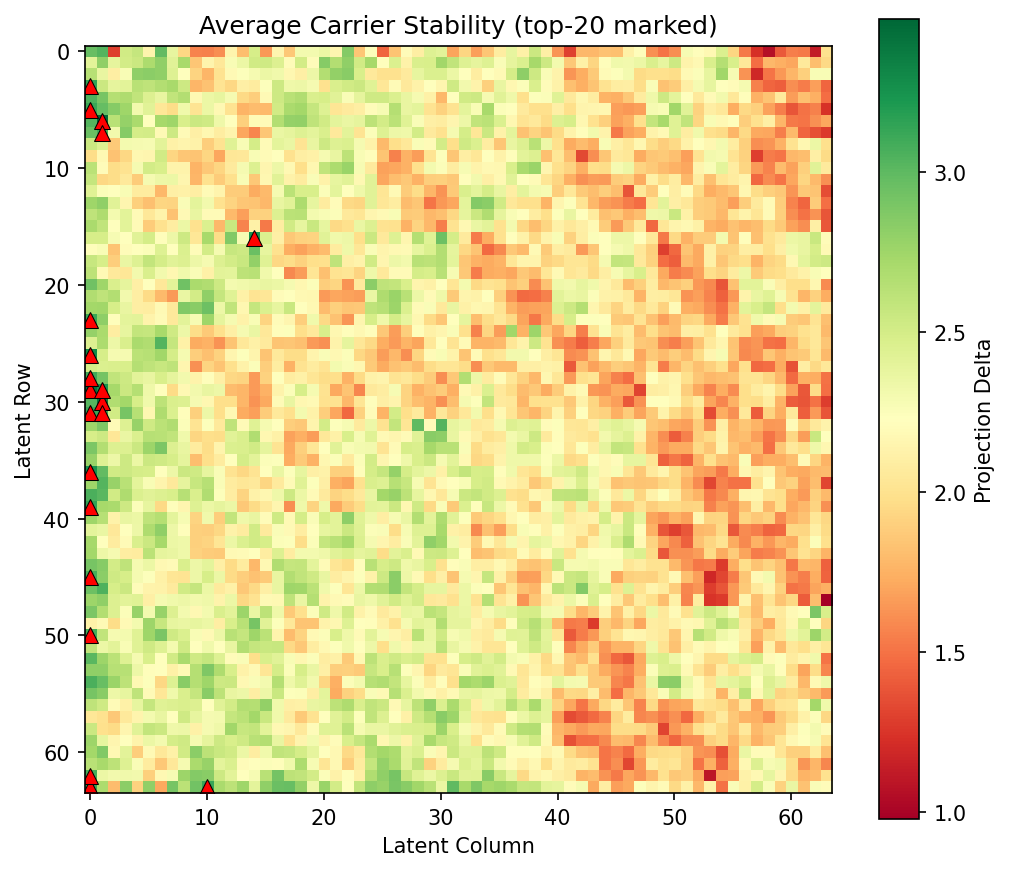
\includegraphics[width=0.78\columnwidth]{figures/carrier_stability_avg.png}
\caption{Average carrier stability map across test images at $\epsilon=5.0$. High-scoring positions preserve perturbation direction more reliably after decode--reencode.}
\label{fig:stability}
\end{figure}

\subsection{Stability Is Content-Dependent}

Content strongly affects stability. Smooth gradients are poor carriers, often near chance even without additional distortion, while color blocks, noise, and natural textured images support reliable recovery. Across 50 synthetic images spanning 10 structural types, entropy and high-frequency energy are among the strongest predictors of capacity, with Pearson correlations of 0.555 and 0.534 respectively.

\begin{figure}[t]
\centering
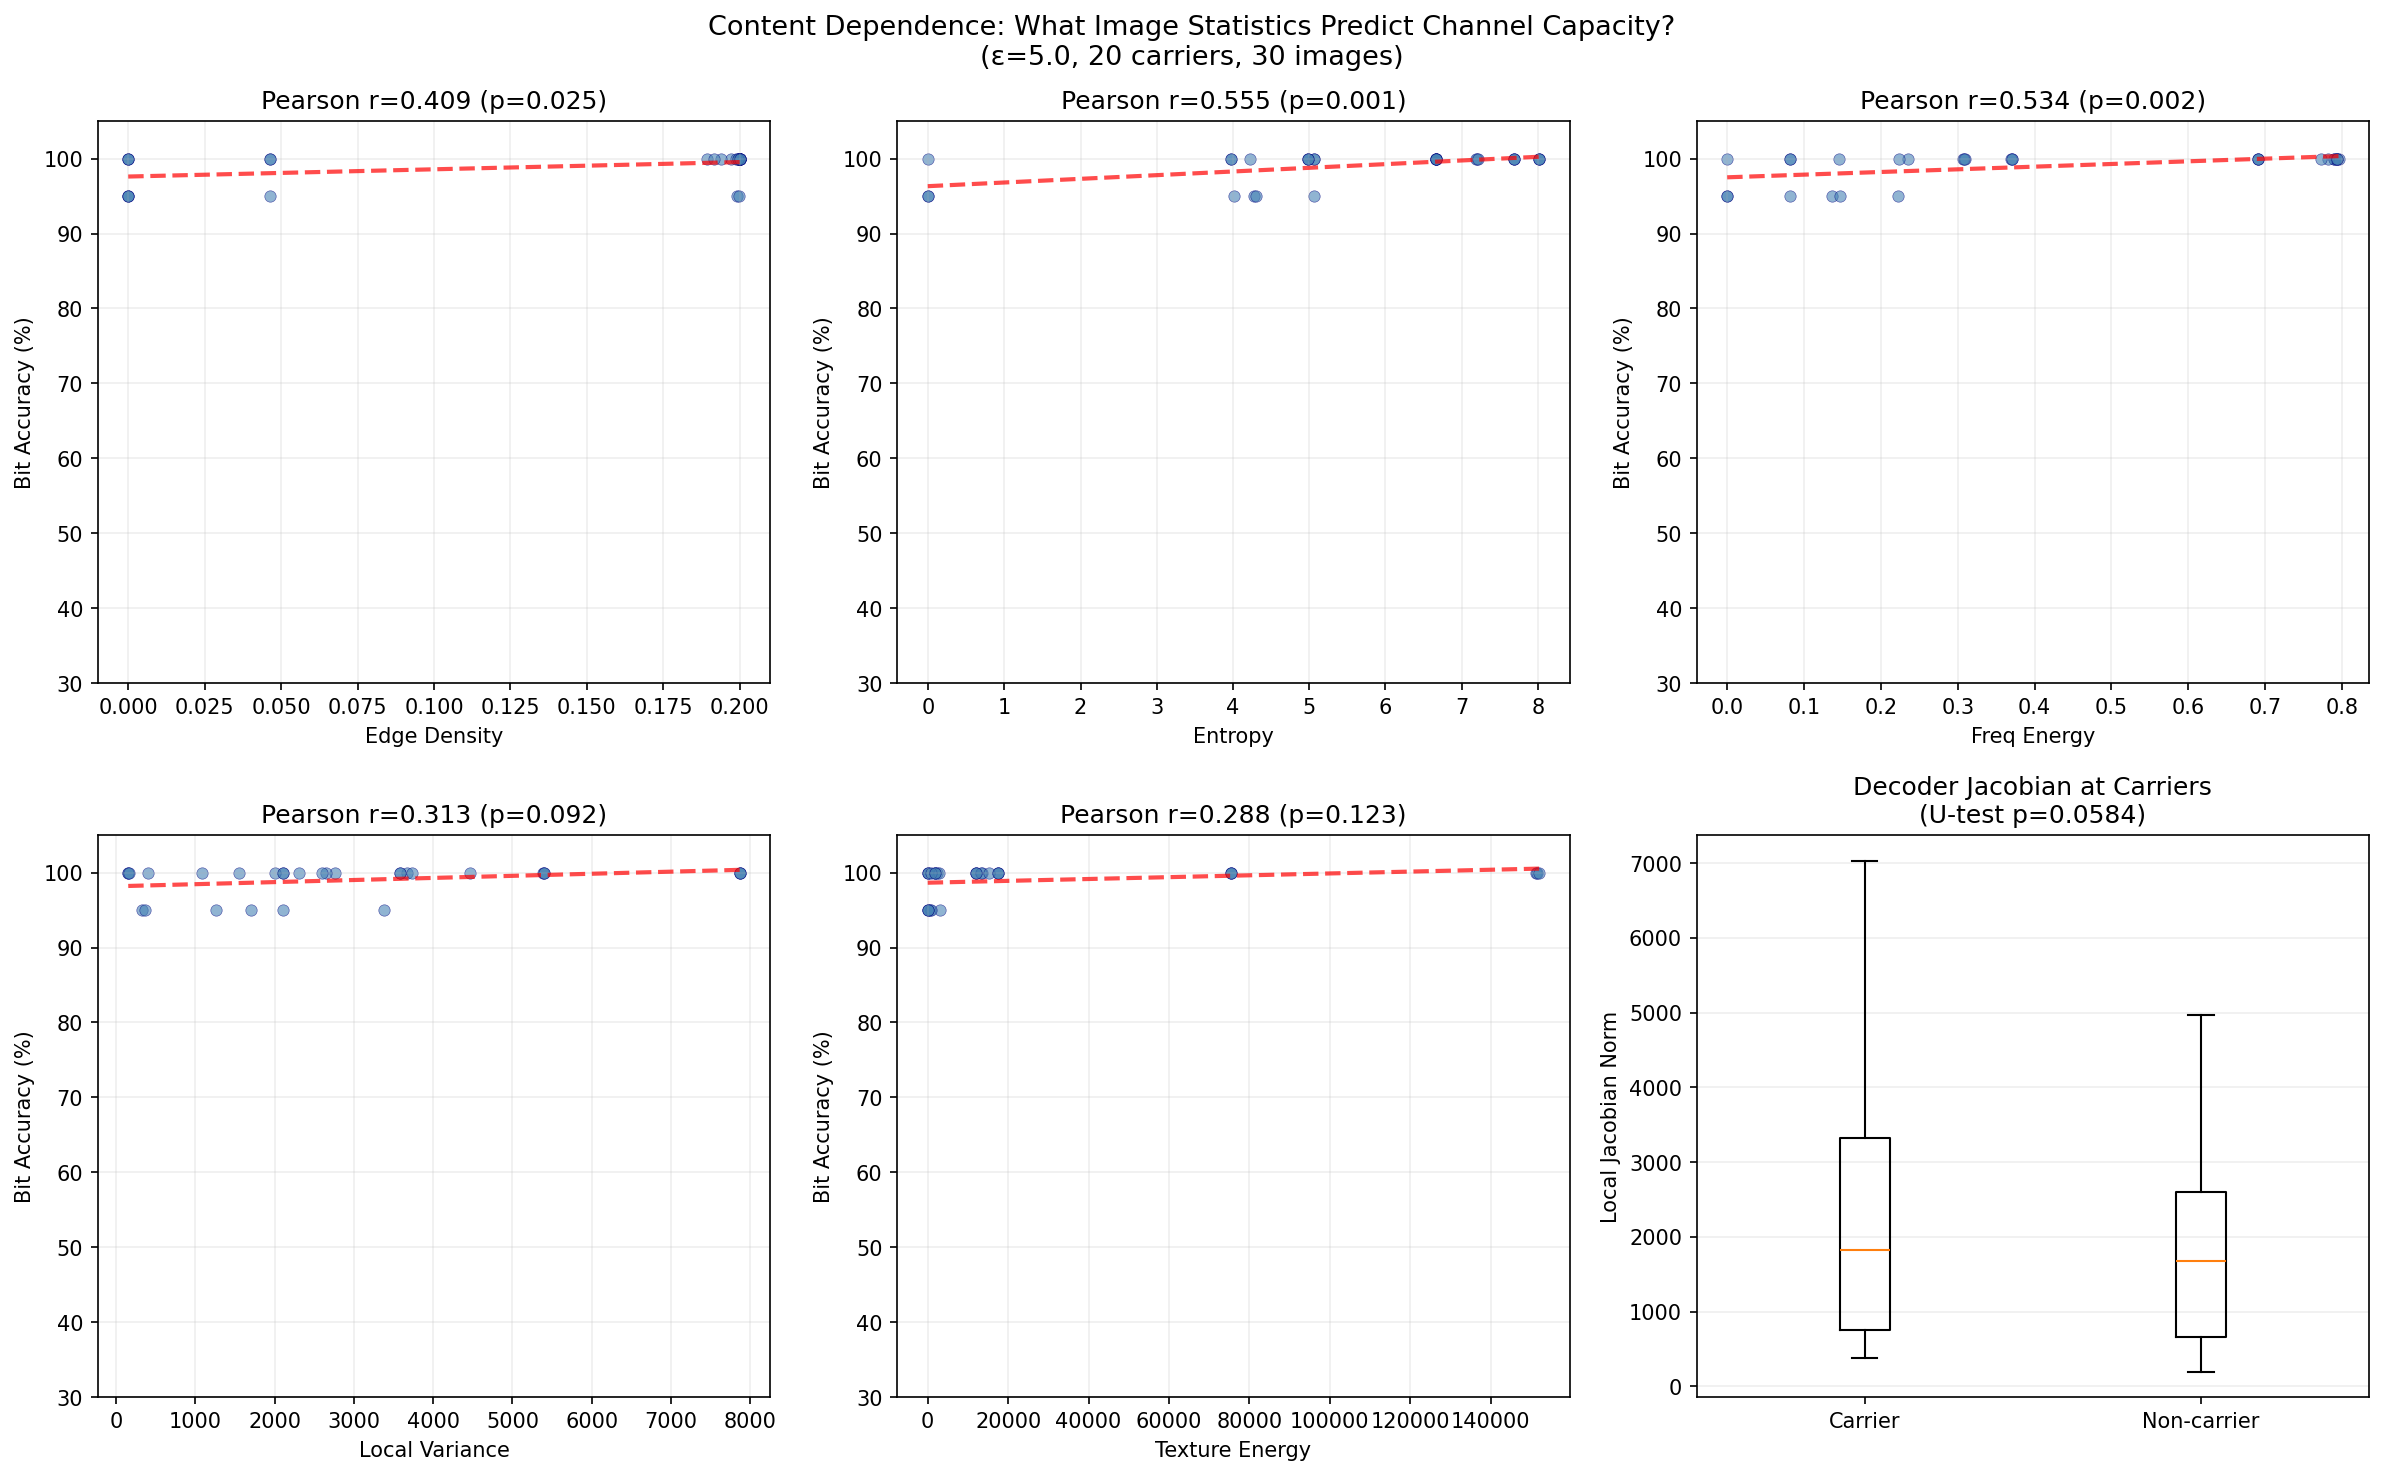
\includegraphics[width=\columnwidth]{figures/content_science.png}
\caption{Content dependence of latent stability. Image statistics such as entropy and high-frequency energy correlate with bit recovery, while finite-difference geometry shows higher local sensitivity at selected carriers.}
\label{fig:content}
\end{figure}

The content dependence suggests that the carrier map is not merely a fixed architectural artifact. Instead, stability is induced by the interaction between image content and local encode--decode geometry. This also explains why smooth images have little usable channel capacity: perturbations are not reliably represented in the re-encoded latent.

\subsection{Natural Images And VAE Backbones}

On 300 CIFAR-10 images, PatchSteg achieves high average recovery with stability-selected carriers: 98.2\% bit accuracy at $\epsilon=2.0$ with 95\% CI [97.8, 98.7], and 98.5\% at $\epsilon=5.0$ with 95\% CI [98.0, 98.9]. The corresponding mean PSNR values are 38.6 dB and 28.9 dB. These results show that the phenomenon is not restricted to toy images, though the use of upscaled CIFAR-10 remains a limitation.

\begin{figure}[t]
\centering
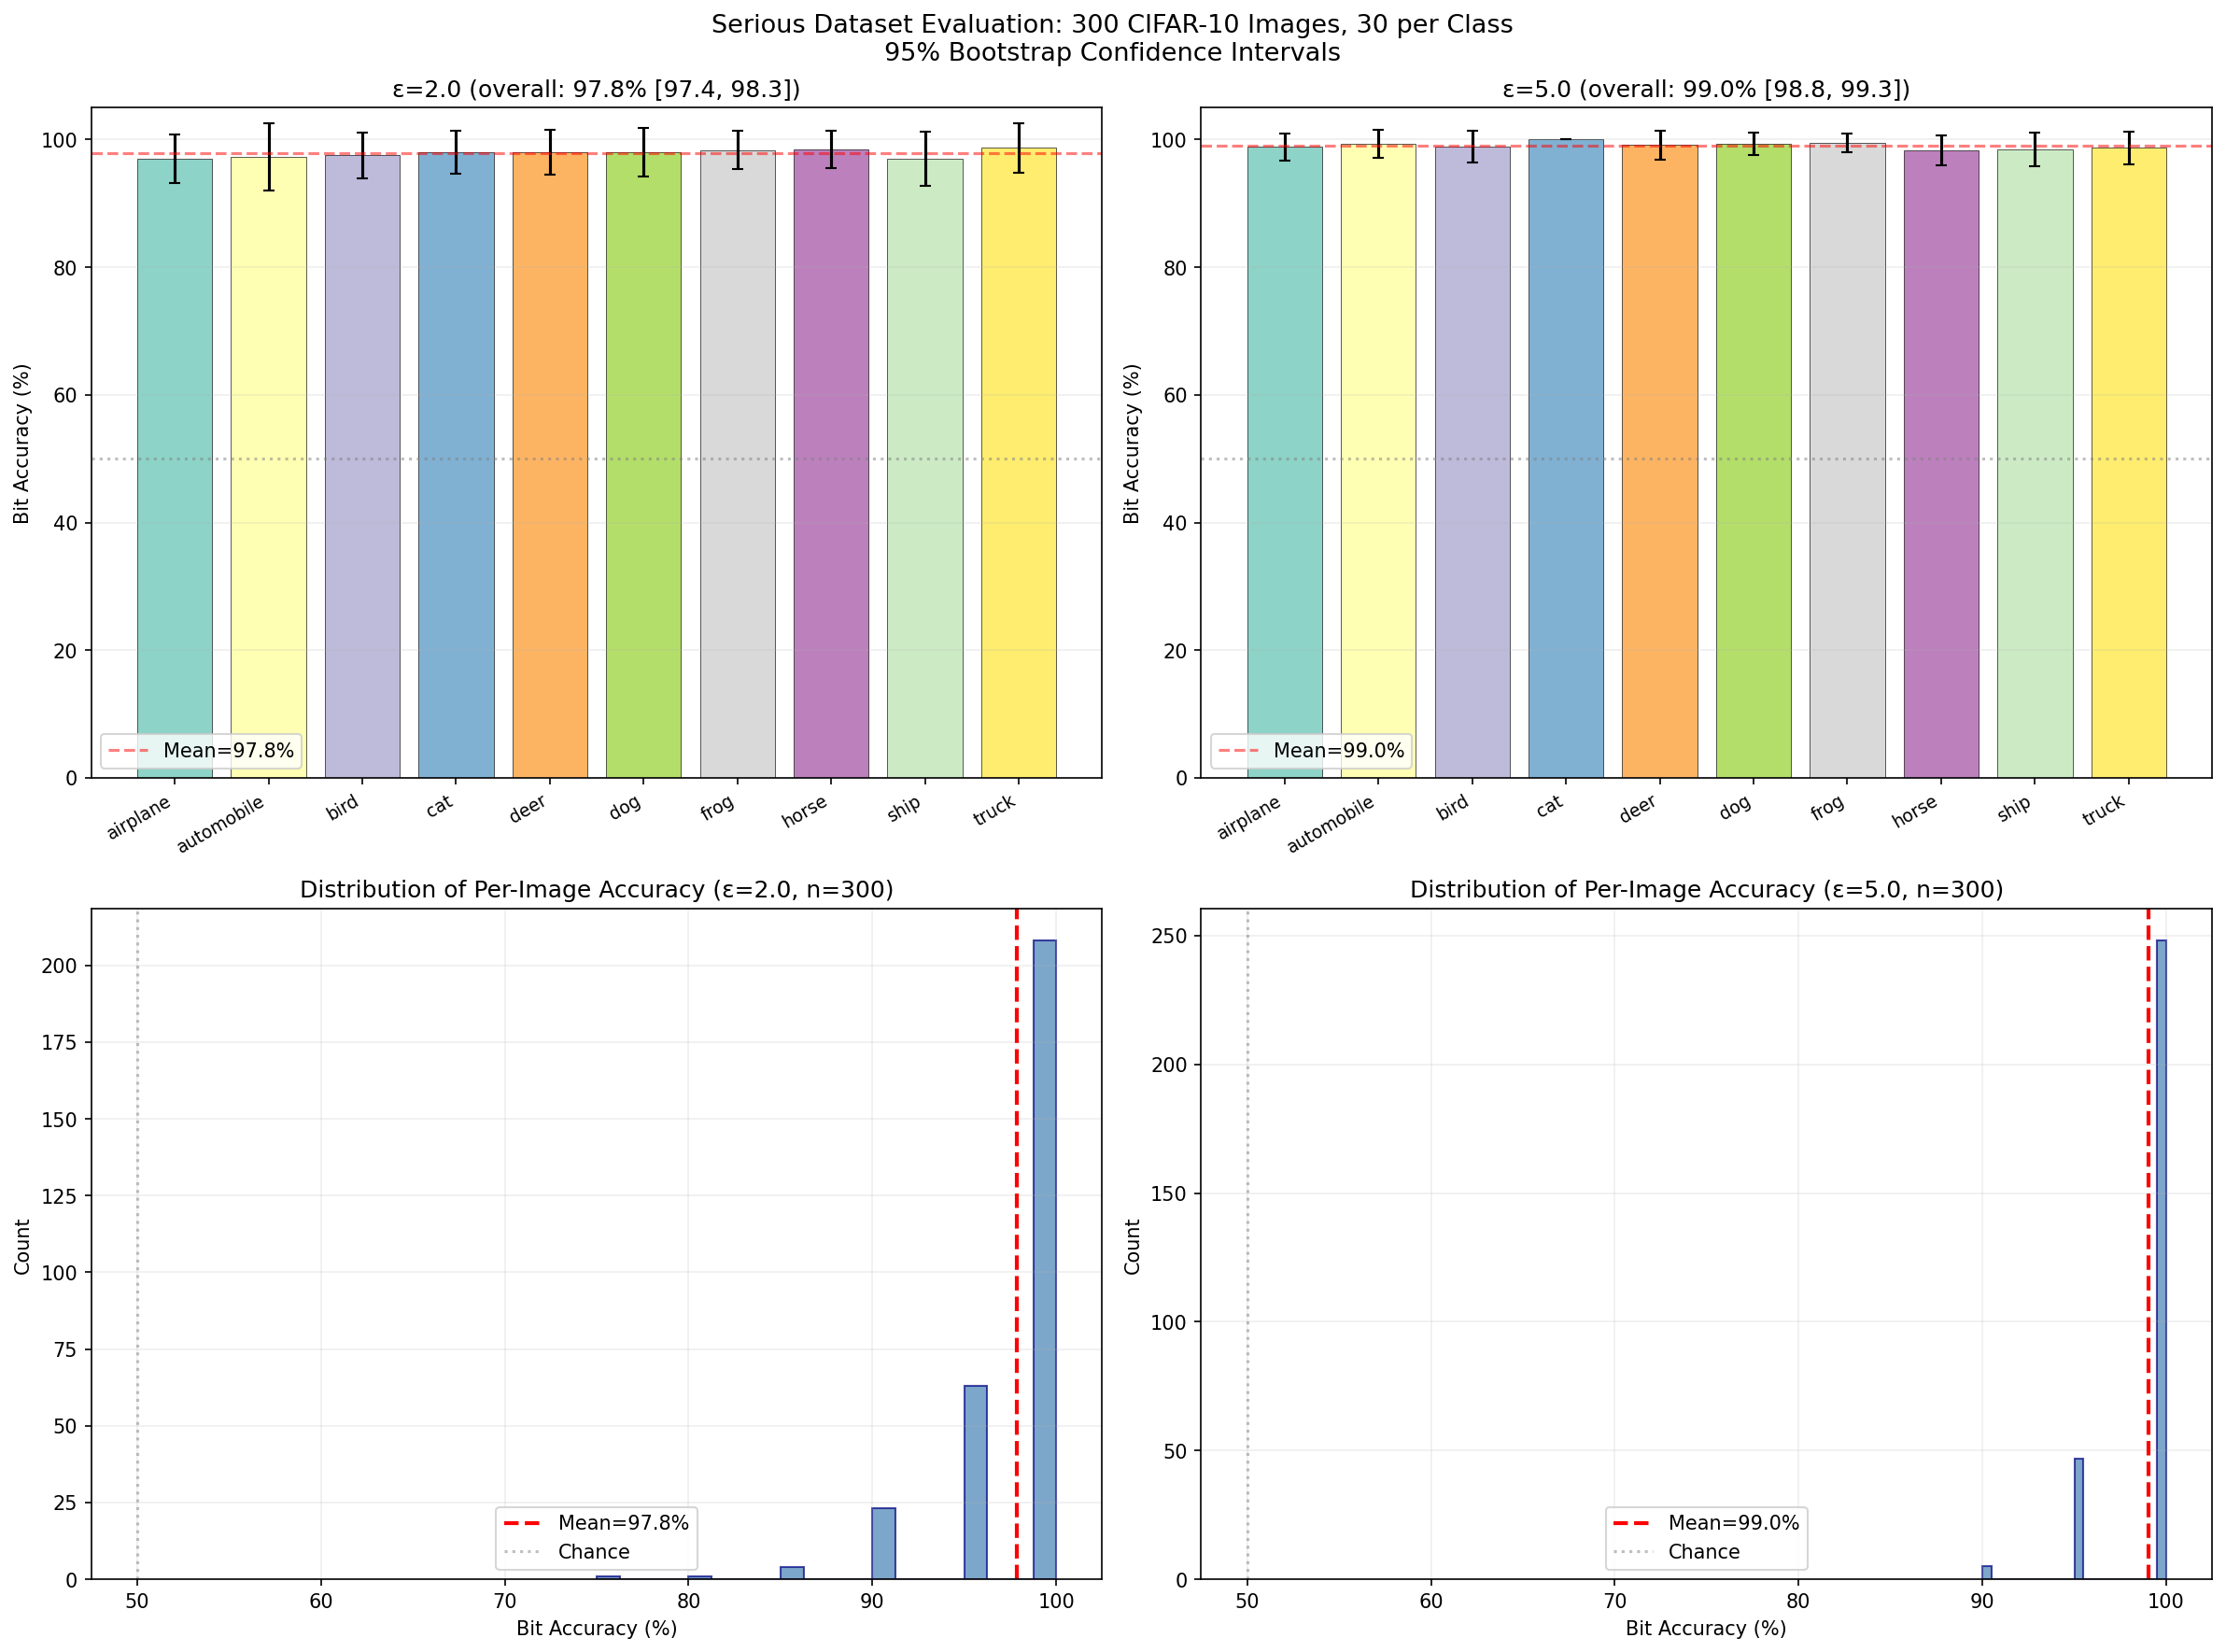
\includegraphics[width=\columnwidth]{figures/serious_dataset.png}
\caption{Evaluation on 300 CIFAR-10 images. Recovery is high across classes, with per-class variation consistent with content-dependent stability.}
\label{fig:natural}
\end{figure}

The probe also generalizes across VAE checkpoints. SD-VAE-MSE, SD-VAE-EMA, and SDXL-VAE all preserve enough local intervention signal for high bit recovery, although SDXL-VAE is weaker at $\epsilon=5.0$ in our current experiment. Cross-model decoding between SD-VAE-MSE and SD-VAE-EMA remains highly accurate, suggesting that some stable directions are shared across related checkpoints.

\begin{figure}[t]
\centering
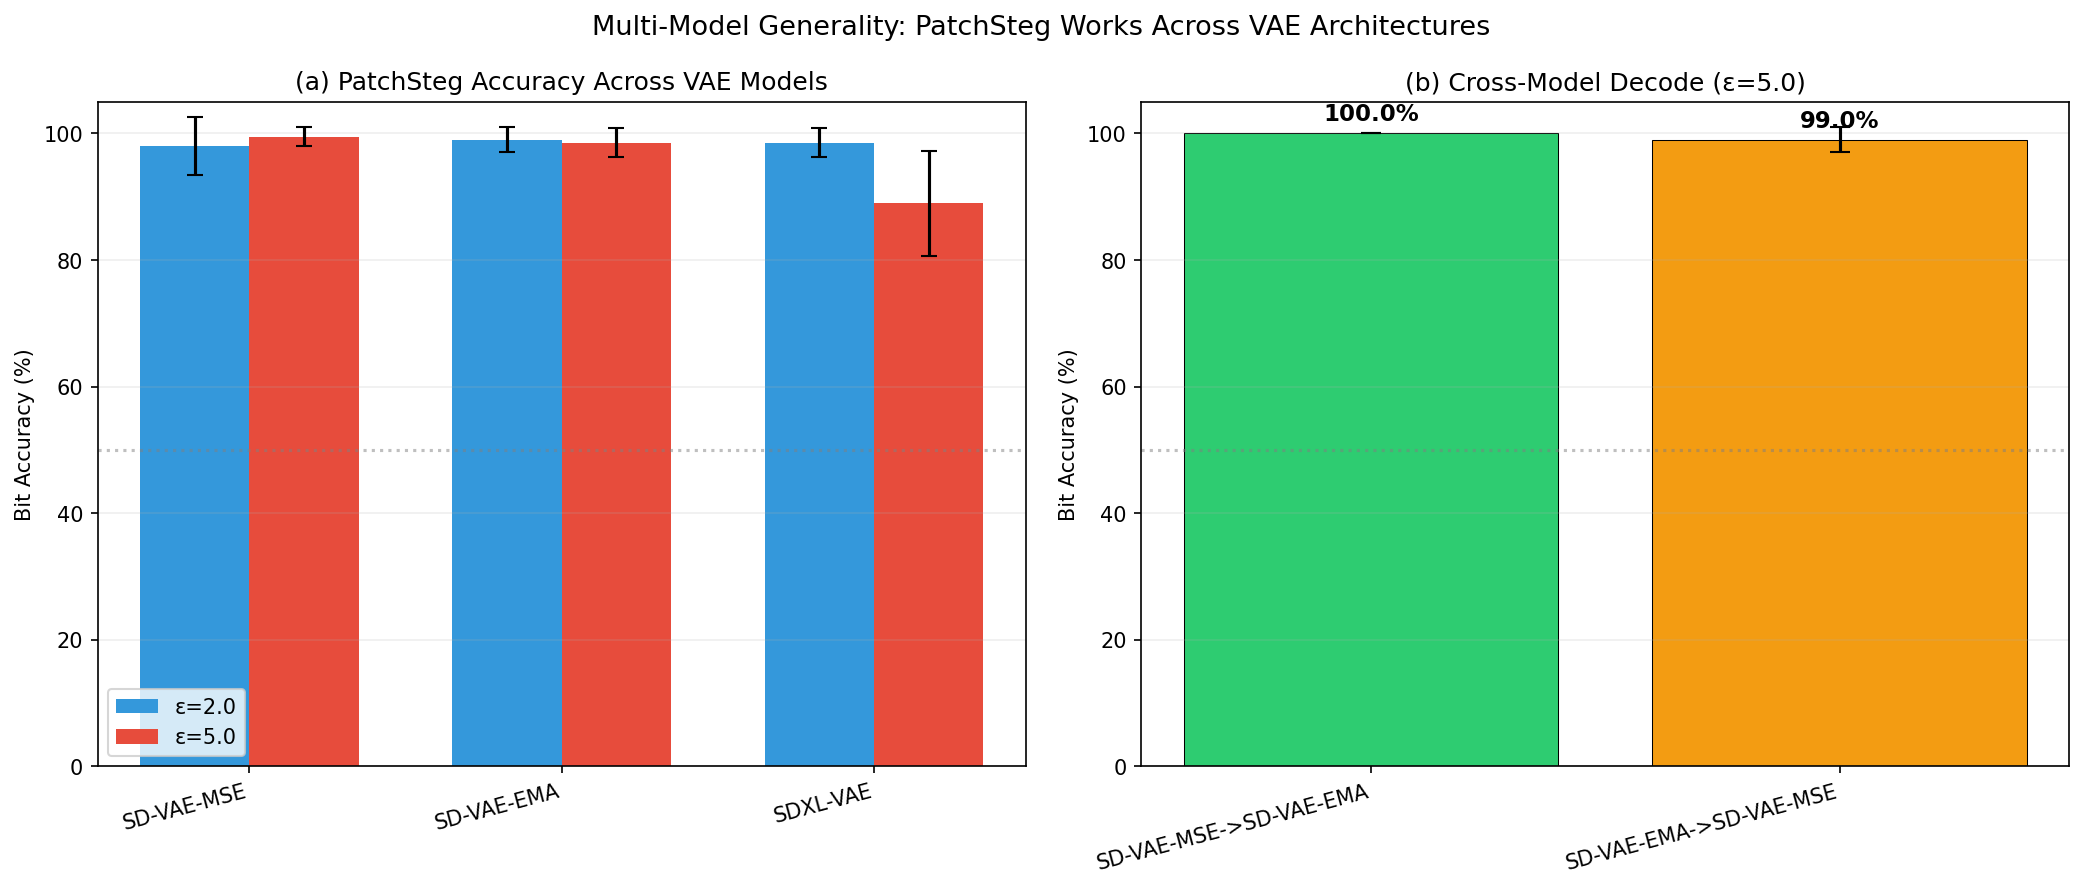
\includegraphics[width=\columnwidth]{figures/multimodel.png}
\caption{PatchSteg recovery across VAE backbones and cross-model encode/decode pairs. The effect is strongest for related Stable Diffusion VAE checkpoints but is not limited to a single model file.}
\label{fig:multimodel}
\end{figure}

\section{Mechanistic Analysis}

\subsection{Reconstruction Error Is Not Carrier Quality}

A natural hypothesis is that stable carriers are simply positions with low reconstruction error. We tested this by comparing baseline reconstruction error against stability and found near-zero correlation: average Pearson $r=0.048$ across images. Thus, the VAE's ability to reconstruct a region faithfully is not the same as its ability to preserve an inserted local perturbation.

\begin{figure}[t]
\centering
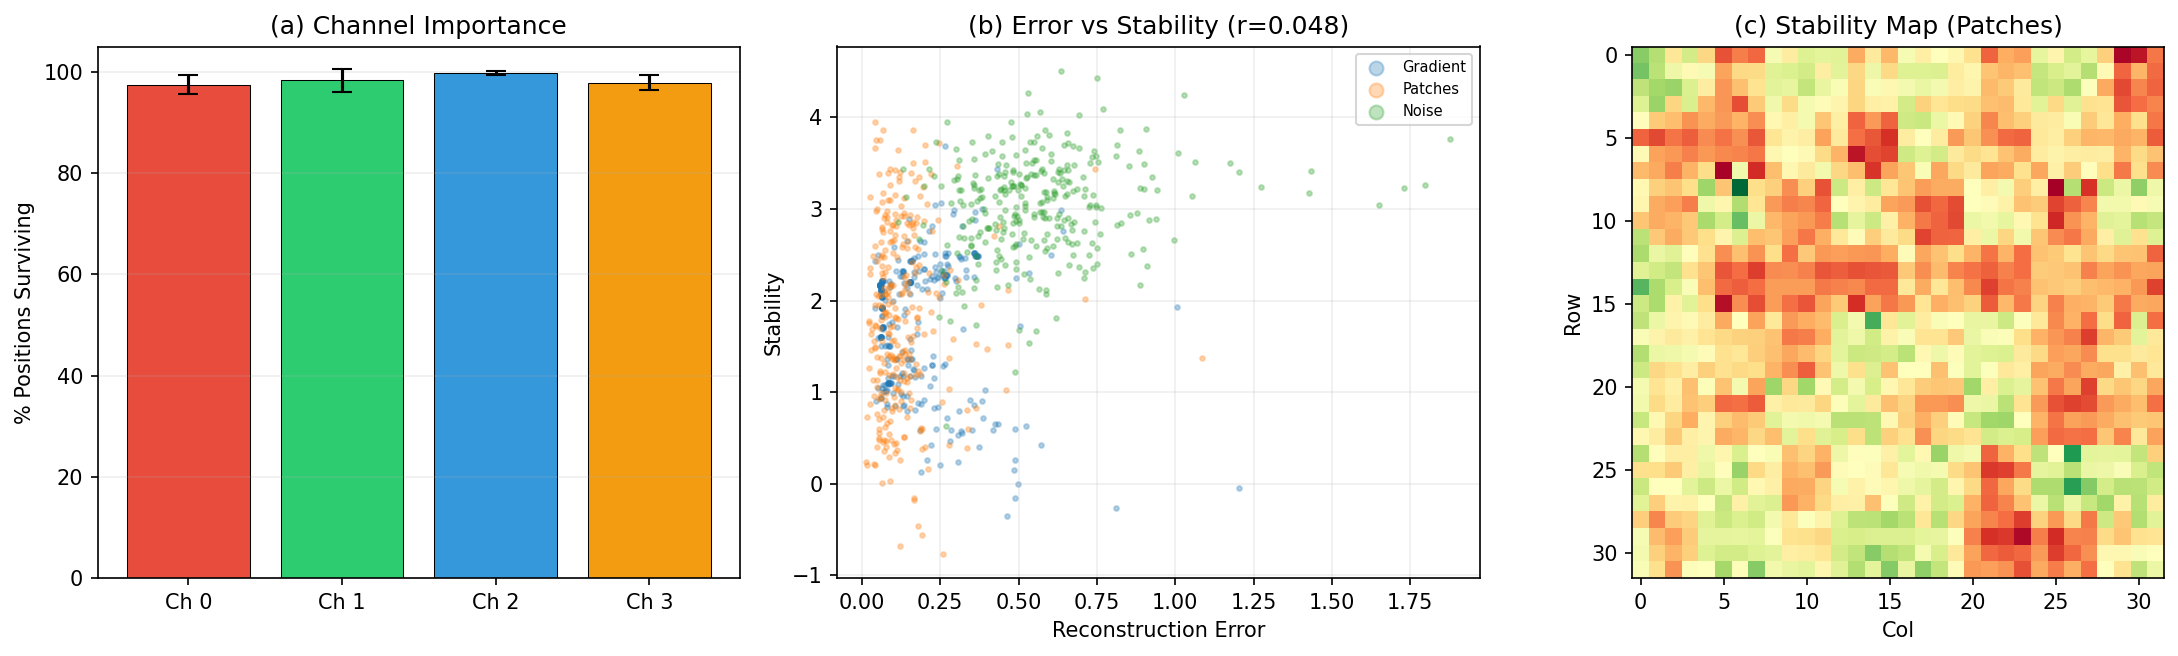
\includegraphics[width=\columnwidth]{figures/mechanistic_analysis.png}
\caption{Mechanistic analysis. All four latent channels contribute to recovery, reconstruction error is weakly correlated with stability, and spatial stability varies substantially within an image.}
\label{fig:mechanistic}
\end{figure}

This distinction matters for interpretability. Reconstruction metrics summarize output fidelity, while stability probes whether an intervention remains encoded in the model's internal state after a round trip. A model can reconstruct an image well while erasing a local signed perturbation, or reconstruct imperfectly while preserving that perturbation's sign.

\subsection{Local Geometry Predicts Stability}

We estimate local decoder sensitivity by finite differences: for each latent position, perturb each of the four channels by $\delta=0.1$ and measure the resulting pixel change. Carrier positions exhibit higher average Jacobian norms than non-carrier positions in the current experiment (2050 vs. 1684, Mann--Whitney $p=0.058$). The evidence is suggestive rather than decisive, but it supports the geometric picture: high-stability positions are locations where the decoder maps latent perturbations into image-space changes that the encoder can recover.

The stronger mechanistic target for future work is the local Jacobian of the composite map $\mathrm{Enc}\circ\mathrm{Dec}$, including singular values and alignment with candidate perturbation directions. PatchSteg supplies a behavioral readout for that geometry; a complete account should predict bit recovery directly from the composite Jacobian.

\subsection{Direction And Channel Structure}

All four latent channels support recovery, with per-channel survival rates between 97.5\% and 99.7\% in our single-channel perturbation experiment. Random direction choices are also robust on structured images at high $\epsilon$, suggesting that the effect is not caused by one uniquely privileged latent channel. We treat this as preliminary evidence for locally broad preservation in the four-channel latent vector, not as a proof of isotropy.

PCA-guided directions provide an additional probe. Perturbing along the top latent principal component yields 100\% accuracy and lower latent-statistics detector AUC than a random direction in a small experiment, while lower-variance components trade off quality and recovery. This is consistent with the idea that data-aligned directions can be more naturally preserved, but the current PCA results are exploratory and should be scaled before making stronger claims.

\section{Safety And Monitoring Implications}

\subsection{Reliability--Stealth Tradeoff}

Because PatchSteg is a signed latent intervention, increasing $\epsilon$ improves recovery while making distribution shifts easier to detect. A latent-statistics logistic regression detector yields AUC 0.44 at $\epsilon=1.0$, 0.68 at $\epsilon=2.0$, and 0.93 at $\epsilon=5.0$ in one 3-fold protocol. Stronger detector families can perform better, especially with pixel-residual and spectral features. We therefore state the monitoring result narrowly: stable latent directions can instantiate a covert channel, but detectability depends heavily on detector class, feature domain, payload strength, and dataset.

\begin{table}[t]
\caption{Representative detection results for latent-statistics logistic regression. These numbers bound only this detector and protocol; stronger feature sets can detect lower perturbation strengths.}
\label{tab:detect}
\centering
\begin{small}
\begin{tabular}{ccc}
\toprule
$\epsilon$ & AUC & Accuracy \\
\midrule
1.0 & $0.440 \pm 0.065$ & $0.467 \pm 0.125$ \\
2.0 & $0.680 \pm 0.113$ & $0.600 \pm 0.082$ \\
5.0 & $0.933 \pm 0.068$ & $0.833 \pm 0.125$ \\
10.0 & $0.973 \pm 0.038$ & $0.900 \pm 0.141$ \\
\bottomrule
\end{tabular}
\end{small}
\end{table}

\subsection{Robustness Under Image Transformations}

The channel can survive realistic distortions when carrier stability is high. In deployment-style tests, $\epsilon=5.0$ survives VAE re-encoding (99\%), screenshot simulation (98.5\%), JPEG Q=10 (96.5\%), resize to 25\% (92\%), and additive noise with $\sigma=0.10$ (98\%). Cropping is more destructive because it changes spatial carrier alignment. This reinforces the interpretation that carrier location and local geometry, not just global image quality, determine recovery.

\section{Exploratory Extensions}
\label{sec:extensions}

The repository contains two extension families that are useful for future work but are not central to the main interpretability claim. First, CDF-PatchSteg replaces carrier values with samples from upper or lower halves of an estimated Gaussian marginal. This removes the clean-cover baseline assumption and is harder for marginal-statistics detectors in small experiments, but current results use only a few images and should be treated as pilot evidence. Second, sanitization experiments, including latent smoothing and quantile reflection, show a fidelity--disruption tradeoff: stronger sanitizers reduce bit recovery but often damage image quality. These results are best understood as preliminary safety probes, not mature defenses.

\section{Limitations}

PatchSteg assumes access to a compatible VAE, and the baseline protocol assumes that sender and receiver share the clean cover or can reproduce its clean round-trip latent. The strongest natural-image evaluation uses CIFAR-10 resized to $256\times256$, which introduces interpolation artifacts and should be supplemented with native high-resolution images. PSNR is an incomplete perceptual metric; future work should include LPIPS, SSIM, and human perceptual checks. Several extension and defense experiments are small-n pilots, so the main paper does not claim broad undetectability or state-of-the-art steganographic performance. Finally, the current mechanistic analysis suggests a role for local geometry but does not yet fully predict stability from the composite encode--decode Jacobian.

\section{Conclusion}

PatchSteg uses bit recovery as a simple intervention-based probe of diffusion VAE latent stability. The main finding is that pretrained VAE latents contain spatially localized, content-dependent directions whose sign survives a round trip through image space. This property enables a bounded covert channel, but more importantly for mechanistic interpretability, it exposes a measurable gap between reconstruction quality and information preservation. Understanding that gap may help characterize how generative autoencoders store, erase, and transmit information through their internal representations.

\bibliography{main}
\bibliographystyle{../icml2026/icml2026}

\appendix

\section{Additional Notes On Claim Scope}

The full repository includes additional payload layers, adaptive pairwise encoding, CDF-style distribution matching, latent detectors, and sanitizers. These components are useful for follow-up research but are intentionally separated from the main workshop claims unless evaluated under the same dataset and detector protocol. The acceptance review log in this directory records the major manuscript changes made for the ICML-style version.

\end{document}
